% ===== FILE: image/diagram.tex =====
% RAPT-CLIP: SOTA Tri-Stream Architecture (CMAF + Unified Temporal Modeling)
% High-Impact Q1 Journal Presentation Grade (IEEE TAC, Information Fusion, Pattern Recognition)
\documentclass[tikz, border=3mm]{standalone}
\usepackage[utf8]{inputenc}
\usepackage{amsmath, amssymb}
\usepackage{graphicx}
\usepackage{xcolor}
\usepackage{tgheros}
\renewcommand{\familydefault}{\sfdefault}
\usetikzlibrary{positioning, arrows.meta, calc, fit, backgrounds, shadows}

% ==============================================================================
% CURATED SCIENTIFIC SOTA PALETTE (Vibrant, Bold & High Contrast)
% ==============================================================================
\definecolor{techNavy}{RGB}{15, 34, 64}
\definecolor{techBlue}{RGB}{37, 99, 235}
\definecolor{techBlueLight}{RGB}{239, 246, 255}
\definecolor{techBlueDark}{RGB}{29, 78, 216}

\definecolor{emeraldGreen}{RGB}{16, 185, 129}
\definecolor{emeraldLight}{RGB}{236, 253, 245}
\definecolor{emeraldDark}{RGB}{5, 150, 105}

\definecolor{cmafAmber}{RGB}{245, 158, 11}
\definecolor{cmafOrange}{RGB}{234, 88, 12}
\definecolor{cmafLight}{RGB}{255, 251, 235}
\definecolor{cmafDark}{RGB}{180, 83, 9}

\definecolor{cosmicPurple}{RGB}{139, 92, 246}
\definecolor{purpleLight}{RGB}{245, 243, 255}
\definecolor{purpleDark}{RGB}{109, 40, 217}

\definecolor{magentaPink}{RGB}{236, 72, 153}
\definecolor{pinkLight}{RGB}{253, 242, 248}
\definecolor{magentaDark}{RGB}{190, 24, 93}

\definecolor{rubyRed}{RGB}{225, 29, 72}
\definecolor{redLight}{RGB}{255, 241, 242}
\definecolor{rubyDark}{RGB}{159, 18, 57}

\definecolor{tealCyan}{RGB}{13, 148, 136}
\definecolor{cyanLight}{RGB}{240, 253, 250}
\definecolor{tealDark}{RGB}{15, 118, 110}

\definecolor{slateGray}{RGB}{100, 116, 139}
\definecolor{grayLight}{RGB}{248, 250, 252}
\definecolor{slateDark}{RGB}{30, 41, 59}

\definecolor{goldAccent}{RGB}{217, 119, 6}

\begin{document}

\begin{tikzpicture}[
    scale=0.58, every node/.style={scale=0.58},
    >={Stealth[length=4.5pt, width=3.2pt]},
    base/.style={draw, rounded corners=4pt, minimum height=1.05cm, align=center,
                 font=\footnotesize, line width=1.0pt,
                 drop shadow={opacity=0.10, shadow xshift=1.2pt, shadow yshift=-1.2pt}},
    bluebox/.style={base, top color=techBlueLight, bottom color=techBlueLight!60!techBlue!35,
                    draw=techBlue!95!techNavy, text=techNavy, text width=2.45cm},
    greenbox/.style={base, top color=emeraldLight, bottom color=emeraldLight!60!emeraldGreen!35,
                     draw=emeraldGreen!95!emeraldDark, text=emeraldDark, text width=2.25cm},
    orangebox/.style={base, top color=purpleLight, bottom color=purpleLight!60!cosmicPurple!35,
                      draw=cosmicPurple!95!purpleDark, text=purpleDark, text width=2.65cm},
    purplebox/.style={base, top color=pinkLight, bottom color=pinkLight!60!magentaPink!35,
                      draw=magentaPink!95!magentaDark, text=magentaDark, text width=2.15cm},
    cyanbox/.style={base, top color=cyanLight, bottom color=cyanLight!60!techBlue!35,
                    draw=tealCyan!90!techNavy, text=techNavy, text width=2.35cm},
    graybox/.style={base, top color=grayLight, bottom color=grayLight!60!slateGray!35,
                    draw=slateGray!90!slateDark, text=slateDark, text width=1.7cm},
    lossbox/.style={base, top color=redLight, bottom color=redLight!60!rubyRed!35,
                    draw=rubyRed!95!rubyDark, text=rubyDark, text width=2.3cm, line width=1.15pt},
    cmafcore/.style={draw=cmafOrange!95!cmafDark, rounded corners=6pt, line width=1.35pt,
                     top color=cmafLight, bottom color=cmafLight!60!cmafAmber!30,
                     drop shadow={opacity=0.16, shadow xshift=1.8pt, shadow yshift=-1.8pt}},
    smallbox/.style={draw=slateGray!60, minimum width=0.7cm, minimum height=0.7cm,
                     rounded corners=2pt, inner sep=0pt, drop shadow={opacity=0.08}},
    flowFace/.style={->, line width=1.2pt, draw=cmafOrange!95!black},
    flowBody/.style={->, line width=1.2pt, draw=techBlue!95!black},
    flowCtx/.style={->, line width=1.2pt, draw=tealCyan!95!black},
    flowMaster/.style={->, line width=1.2pt, draw=slateDark!85},
    darr/.style={->, line width=1.25pt, draw=rubyRed!95!black, dashed},
]

% ====================================================================
%                        VISUAL BRANCH (TRI-STREAM CMAF SOTA)
% ====================================================================

% --- Stream 1: Face Input (F_{1..T}) ---
\node[inner sep=1.2pt, draw=cmafOrange!80, line width=1.0pt, rounded corners=3pt, drop shadow={opacity=0.25}] 
    (f3) at (-1.0, 3.25) {
\includegraphics[width=2.2cm, height=2.2cm]{input_face.jpg}};
\node[inner sep=1.2pt, draw=cmafOrange!85, line width=1.0pt, rounded corners=3pt, drop shadow={opacity=0.25}] 
    (f2) at (-0.5, 3.60) {
\includegraphics[width=2.2cm, height=2.2cm]{input_face.jpg}};
\node[inner sep=1.2pt, draw=cmafOrange!95!black, line width=1.15pt, rounded corners=3pt, drop shadow={opacity=0.3}] 
    (f1) at (0.0, 3.95) {
\includegraphics[width=2.2cm, height=2.2cm]{input_face.jpg}};
\node[fill=cmafOrange!15, draw=cmafOrange!70, rounded corners=2.5pt, font=\scriptsize\bfseries, text=cmafDark, inner sep=2.5pt] 
    at (-0.5, 5.45) {Face Stream: $F_{1,2,\dots,T}$};

% --- Stream 2: Body Input (B_{1..T}) ---
\node[inner sep=1.2pt, draw=techBlue!80, line width=1.0pt, rounded corners=3pt, drop shadow={opacity=0.25}] 
    (b3) at (-1.0, -0.35) {
\includegraphics[width=2.2cm, height=2.2cm]{input_body.jpg}};
\node[inner sep=1.2pt, draw=techBlue!85, line width=1.0pt, rounded corners=3pt, drop shadow={opacity=0.25}] 
    (b2) at (-0.5, 0.00) {
\includegraphics[width=2.2cm, height=2.2cm]{input_body.jpg}};
\node[inner sep=1.2pt, draw=techBlue!95!black, line width=1.15pt, rounded corners=3pt, drop shadow={opacity=0.3}] 
    (b1) at (0.0, 0.35) {
\includegraphics[width=2.2cm, height=2.2cm]{input_body.jpg}};
\node[fill=techBlueLight, draw=techBlue!65, rounded corners=2.5pt, font=\scriptsize\bfseries, text=techBlueDark, inner sep=2.5pt] 
    at (-0.5, 1.85) {Body Stream: $B_{1,2,\dots,T}$};

% --- Stream 3: Context Input (C_{1..T}) ---
\node[inner sep=1.2pt, draw=tealCyan!80, line width=1.0pt, rounded corners=3pt, drop shadow={opacity=0.25}] 
    (c3) at (-1.0, -3.95) {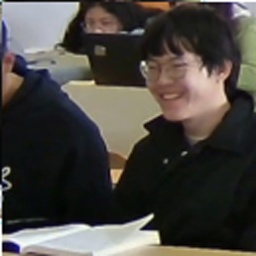
\includegraphics[width=2.2cm, height=2.2cm]{input_context.jpg}};
\node[inner sep=1.2pt, draw=tealCyan!85, line width=1.0pt, rounded corners=3pt, drop shadow={opacity=0.25}] 
    (c2) at (-0.5, -3.60) {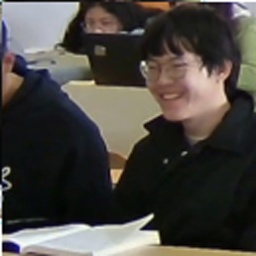
\includegraphics[width=2.2cm, height=2.2cm]{input_context.jpg}};
\node[inner sep=1.2pt, draw=tealCyan!95!black, line width=1.15pt, rounded corners=3pt, drop shadow={opacity=0.3}] 
    (c1) at (0.0, -3.25) {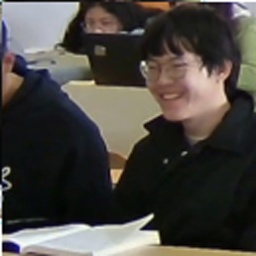
\includegraphics[width=2.2cm, height=2.2cm]{input_context.jpg}};
\node[fill=cyanLight, draw=tealCyan!65, rounded corners=2.5pt, font=\scriptsize\bfseries, text=tealDark, inner sep=2.5pt] 
    at (-0.5, -1.75) {Context Stream: $C_{1,2,\dots,T}$};

% --- CLIP Image Encoders (Shared ViT-B/16 Weights, Frozen) ---
\node[bluebox, font=\normalsize] (fenc) at (3.5, 3.6) {
    \textbf{CLIP ViT-B/16}\\[2pt]
    {\scriptsize (Backbone, Frozen)}\\[1pt]
    {\tiny\texttt{out: $512\text{-d}$}}
};
\node[bluebox, font=\normalsize] (benc) at (3.5, 0.0) {
    \textbf{CLIP ViT-B/16}\\[2pt]
    {\scriptsize (Backbone, Frozen)}\\[1pt]
    {\tiny\texttt{out: $512\text{-d}$}}
};
\node[bluebox, font=\normalsize] (cenc) at (3.5, -3.6) {
    \textbf{CLIP ViT-B/16}\\[2pt]
    {\scriptsize (Backbone, Frozen)}\\[1pt]
    {\tiny\texttt{out: $512\text{-d}$}}
};

% Shared Weights Badges
\draw[dashed, slateGray!75, line width=1.0pt] (fenc.south) -- 
    node[fill=white, draw=techBlue!50, rounded corners=2pt, inner sep=1.8pt, font=\tiny\bfseries, text=techBlueDark] {Shared $\theta_{\text{ViT}}$} (benc.north);
\draw[dashed, slateGray!75, line width=1.0pt] (benc.south) -- 
    node[fill=white, draw=techBlue!50, rounded corners=2pt, inner sep=1.8pt, font=\tiny\bfseries, text=techBlueDark] {Shared $\theta_{\text{ViT}}$} (cenc.north);

% --- Face Adapter (EAA - Expression-Aware Adapter) ---
\node[greenbox, font=\normalsize] (fadapt) at (6.8, 3.6) {
    \textbf{Face Adapter}\\[1.5pt]
    {\scriptsize\textbf{(EAA)}}\\[2pt]
    {\tiny $512 \!\rightarrow\! 128 \!\rightarrow\! 512$}\\[1pt]
    {\tiny Residual $\Delta\theta_{\text{FER}}$}
};

% ====================================================================
%     FRAME-LEVEL CROSS-MODAL ATTENTION FUSION (CMAF CORE)
% ====================================================================
% CMAF Outer Glassmorphism Container
\node[cmafcore, minimum width=4.3cm, minimum height=8.8cm] (cmaf) at (10.4, 0.0) {};

% CMAF Container Title
\node[anchor=north, font=\large\bfseries, text=cmafDark, yshift=-0.28cm] at (cmaf.north) {CMAF Core};
\node[anchor=north, font=\scriptsize\bfseries, text=cmafOrange!90!black, yshift=-0.78cm] at (cmaf.north) {Tridirectional Cross-Attention};

% Micro-Attention Cards inside CMAF Core
\node[fill=white, draw=cmafOrange!85, line width=0.9pt, rounded corners=3pt, 
      text width=3.65cm, align=center, inner sep=3.5pt, drop shadow={opacity=0.08}] 
      (cmaf_f) at (10.4, 1.95) {
    \textbf{\scriptsize Face Cross-Attention}\\[1pt]
    {\scriptsize $Q_F \otimes [K_B, K_C] \rightarrow \mathbf{f}_t^{\prime F}$}
};

\node[fill=white, draw=techBlue!85, line width=0.9pt, rounded corners=3pt, 
      text width=3.65cm, align=center, inner sep=3.5pt, drop shadow={opacity=0.08}] 
      (cmaf_b) at (10.4, 0.0) {
    \textbf{\scriptsize Body Cross-Attention}\\[1pt]
    {\scriptsize $Q_B \otimes [K_F, K_C] \rightarrow \mathbf{b}_t^{\prime B}$}
};

\node[fill=white, draw=tealCyan!85, line width=0.9pt, rounded corners=3pt, 
      text width=3.65cm, align=center, inner sep=3.5pt, drop shadow={opacity=0.08}] 
      (cmaf_c) at (10.4, -1.95) {
    \textbf{\scriptsize Context Cross-Attention}\\[1pt]
    {\scriptsize $Q_C \otimes [K_F, K_B] \rightarrow \mathbf{c}_t^{\prime C}$}
};

% CMAF Bottom Status
\node[anchor=south, font=\scriptsize\bfseries, text=cmafDark, align=center, yshift=0.25cm] at (cmaf.south) {
    LayerNorm \& Residual Gating\\[1.5pt]
    {\tiny\texttt{Frame-Level Output: $3 \times 512\text{-d}$}}
};

% ====================================================================
%       INTERMEDIATE 3-STAGE BRIDGING & TEMPORAL MODELING
% ====================================================================
% Stage 1: Channel Concatenation (1536-d)
\node[circle, draw=cmafOrange!90!black, top color=cmafAmber!35, bottom color=cmafOrange!45, line width=1.2pt, 
      inner sep=3.5pt, font=\large\bfseries, text=cmafDark, drop shadow={opacity=0.15}] (concat) at (13.6, 0.0) {\textbf{c}};
\node[font=\scriptsize\bfseries, text=cmafDark, below=0.12cm of concat] {1536-d};

% Stage 2: Temporal Positional Addition
\node[circle, draw=cosmicPurple!90!black, top color=purpleLight, bottom color=cosmicPurple!40, line width=1.2pt, 
      inner sep=2.2pt, font=\Large\bfseries, text=purpleDark, drop shadow={opacity=0.15}] (posadd) at (15.5, 0.0) {$\oplus$};
\node[base, top color=purpleLight, bottom color=purpleLight!70!cosmicPurple!30, draw=cosmicPurple!75, 
      font=\scriptsize, text width=1.75cm, text=purpleDark, above=0.55cm of posadd] (posemb) {
    \textbf{Temporal Pos.}\\
    $\mathbf{E}_{\text{pos}} \in \mathbb{R}^{16 \times 1536}$
};

% Stage 3: Unified Temporal Transformer
\node[orangebox, font=\normalsize, text width=2.65cm] (utemp) at (18.3, 0.0) {
    \textbf{Unified Temporal}\\[-1pt]
    \textbf{Transformer}\\[2pt]
    {\scriptsize 1 Layer, $T=16$, $h=8$}\\[1pt]
    {\tiny Pre-LN + MHSA + FFN}
};

% Attention Pooling (Dynamic Frame Weighting)
\node[purplebox, font=\normalsize, text width=2.15cm] (apool) at (21.5, 0.0) {
    \textbf{Attention}\\[-1pt]
    \textbf{Pooling}\\[2pt]
    {\scriptsize $\sum_{t=1}^{16} \alpha_t \mathbf{h}_t$}\\[1pt]
    {\tiny Learnable Weights $\alpha_t$}
};

% Clip-level Visual Representation Vector v
\node[circle, draw=goldAccent!95!black, top color=goldAccent!25, bottom color=goldAccent!55, line width=1.3pt, 
      inner sep=3.2pt, font=\large\bfseries, text=slateDark, drop shadow={opacity=0.2}] (vF) at (23.7, 0.0) {$\mathbf{v}$};
\node[font=\tiny\ttfamily, text=slateDark, below=0.1cm of vF] {(B, 1536)};

% Linear Projection Head (FC 1536 -> 512)
\node[graybox, font=\normalsize] (fc) at (25.9, 0.0) {
    \textbf{Project FC}\\[2pt]
    {\scriptsize $1536 \!\rightarrow\! 512$}\\[1pt]
    {\tiny $+ \ell_2\text{-norm}$}
};

% Primary Task Classification Loss
\node[lossbox, font=\normalsize, text width=2.3cm] (ldamloss) at (28.75, 0.0) {
    \textbf{Task Loss}\\[2pt]
    {\scriptsize\textbf{(LDAM / ASL)}}\\[1pt]
    {\tiny Single / Multi-label}
};

% --- Visual Flow Connections ---
\draw[flowFace] (f1.east) -- (fenc.west);
\draw[flowFace] (fenc) -- (fadapt);
\draw[flowFace] (fadapt.east) -- (cmaf_f.west);

\draw[flowBody] (b1.east) -- (benc.west);
\draw[flowBody] (benc.east) -- (cmaf_b.west);

\draw[flowCtx] (c1.east) -- (cenc.west);
\draw[flowCtx] (cenc.east) -- (cmaf_c.west);

% Tridirectional Convergence into Concat
\draw[flowFace] (cmaf_f.east) -- ++(0.4, 0) |- (concat.north);
\draw[flowBody] (cmaf_b.east) -- (concat.west);
\draw[flowCtx] (cmaf_c.east) -- ++(0.4, 0) |- (concat.south);

% Main Pipeline Flow
\draw[flowMaster] (concat) -- (posadd);
\draw[flowMaster] (posemb) -- (posadd);
\draw[flowMaster] (posadd) -- (utemp);
\draw[flowMaster] (utemp) -- (apool);
\draw[flowMaster] (apool) -- (vF);
\draw[flowMaster] (vF) -- (fc);
\draw[flowMaster] (fc) -- (ldamloss);

% ===== Glassmorphism Visual Branch Enclosure =====
\begin{scope}[on background layer]
    \draw[fill=techBlueLight!30, draw=techBlue!40, rounded corners=10pt, line width=1.2pt] 
        (-2.8, -5.6) rectangle (30.3, 7.3);
    \node[anchor=north west, fill=techNavy, text=white, rounded corners=3.5pt, font=\normalsize\bfseries, inner sep=4.5pt,
          drop shadow={opacity=0.18}] 
        at (-2.3, 6.8) 
        {\quad Visual Branch: Tri-Stream Spatio-Temporal Encoding \& Cross-Modal Attention Fusion (CMAF) \quad};
\end{scope}

% ====================================================================
%            DEDICATED CONTRASTIVE ALIGNMENT CORRIDOR
% ====================================================================
\node[lossbox, top color=redLight, bottom color=redLight!60!rubyRed!35, draw=rubyRed!90!black, 
      line width=1.2pt, text width=5.2cm] (clip_align) at (21.2, -6.55) {
    \textbf{Contrastive Alignment Loss}\\[1.5pt]
    {\scriptsize $\mathcal{L}_{\text{CLIP}} = -\log \frac{\exp(\mathbf{v}^\top \overline{t}_y / \tau)}{\sum_j \exp(\mathbf{v}^\top \overline{t}_j / \tau)}$}
};

% Connections to Contrastive Alignment
\draw[darr, rounded corners=6pt] (fc.south) |- (clip_align.east);

% ====================================================================
%                        TEXT BRANCH (DUAL-VIEW SOTA)
% ====================================================================

% ---- PROMPT ENSEMBLE GROUP ----
\node[draw=cmafOrange!40, rounded corners=4pt, top color=redLight, bottom color=redLight!50!cmafLight!50, 
      text width=3.2cm, align=left, font=\normalsize, inner sep=6pt, drop shadow={opacity=0.08}] 
      (pe1) at (0, -10.0) {
    \textbf{1. Neutrality}\\[1pt]
    {\scriptsize prompt\_1, prompt\_2, \dots}
};
\node[draw=techBlue!40, rounded corners=4pt, top color=techBlueLight, bottom color=techBlueLight!50!purpleLight!50, 
      text width=3.2cm, align=left, font=\normalsize, inner sep=6pt, drop shadow={opacity=0.08}] 
      (pek) at (0, -12.0) {
    \textbf{k. Distraction}\\[1pt]
    {\scriptsize prompt\_1, prompt\_2, \dots}
};
\begin{scope}[on background layer]
    \node[fit=(pe1)(pek), top color=cmafLight!60, bottom color=cmafLight!20, draw=cmafOrange!30, 
          rounded corners=5pt, inner xsep=26pt, inner ysep=34pt,
          label={[font=\normalsize\bfseries, text=cmafDark]below=1pt:Prompt Ensemble}] (pebg) {};
\end{scope}

% ---- Tokenizer ----
\node[base, top color=cmafAmber!20, bottom color=cmafAmber!40, draw=cmafAmber!90!black, 
      text width=2.0cm, font=\normalsize\bfseries, text=slateDark] (tok) at (3.8, -11.0) {Tokenizer};

% ---- Learnable Prompt (CoOp) ----
\node[font=\bfseries, text=cmafDark] at (6.5, -12.0) {Learnable Prompt};
\node[smallbox, top color=cmafAmber!30, bottom color=cmafOrange!40, draw=cmafOrange!80] (lp11) at (6.0, -12.6) {\tiny $v_1$};
\node[smallbox, top color=cmafAmber!40, bottom color=cmafOrange!55, draw=cmafOrange!85] (lp12) at (6.8, -12.6) {\tiny $v_2$};
\node[smallbox, top color=cmafAmber!35, bottom color=cmafOrange!45, draw=cmafOrange!80] (lp21) at (6.0, -13.4) {\tiny $v_3$};
\node[smallbox, top color=cmafAmber!50, bottom color=cmafOrange!65, draw=cmafOrange!90] (lp22) at (6.8, -13.4) {\tiny $v_M$};
\node[draw=cmafOrange!40, rounded corners=3pt, fit=(lp11)(lp12)(lp21)(lp22), inner sep=4pt] (lpbox) {};

% ---- Text Concat ----
\node[circle, draw=cmafOrange!90!black, top color=cmafAmber!35, bottom color=cmafOrange!45, line width=1.1pt, 
      inner sep=3.5pt, font=\large\bfseries, text=cmafDark, drop shadow={opacity=0.15}] (tcat) at (8.4, -11.0) {\textbf{c}};

% ---- CLIP Text Encoder ----
\node[cyanbox, minimum height=8.4cm, text width=2.25cm, font=\normalsize] (tenc) at (11.0, -13.7) {
    \textbf{CLIP}\\[-1pt]
    \textbf{Text}\\[-1pt]
    \textbf{Encoder}\\[3pt]
    {\tiny (Frozen Transformers)}\\[2pt]
    {\tiny\texttt{out: $512\text{-d}$}}
};

% ---- Output Vectors View 1 ----
\node[smallbox, top color=cmafAmber!25, bottom color=cmafOrange!35, draw=cmafOrange!80, minimum width=0.95cm, minimum height=0.95cm, font=\large] (ft1a) at (13.8, -9.9) {$\overline{t}_1^{(1)}$};
\node[smallbox, top color=cmafAmber!25, bottom color=cmafOrange!35, draw=cmafOrange!80, minimum width=0.95cm, minimum height=0.95cm, font=\large] (ft2a) at (13.8, -11.0) {$\overline{t}_2^{(1)}$};
\node[font=\large, text=slateGray] at (13.8, -11.8) {$\vdots$};
\node[smallbox, top color=cmafAmber!25, bottom color=cmafOrange!35, draw=cmafOrange!80, minimum width=0.95cm, minimum height=0.95cm, font=\large] (ftka) at (13.8, -12.7) {$\overline{t}_k^{(1)}$};

% ---- Output Vectors View 2 ----
\node[smallbox, top color=techBlueLight!60, bottom color=techBlue!40, draw=techBlue!80, minimum width=0.95cm, minimum height=0.95cm, font=\Large] (ft1b) at (13.8, -14.4) {$t_1^{(2)}$};
\node[smallbox, top color=techBlueLight!60, bottom color=techBlue!40, draw=techBlue!80, minimum width=0.95cm, minimum height=0.95cm, font=\Large] (ft2b) at (13.8, -15.5) {$t_2^{(2)}$};
\node[font=\large, text=slateGray] at (13.8, -16.4) {$\vdots$};
\node[smallbox, top color=techBlueLight!60, bottom color=techBlue!40, draw=techBlue!80, minimum width=0.95cm, minimum height=0.95cm, font=\Large] (ftkb) at (13.8, -17.4) {$t_k^{(2)}$};

% ---- VIEW 1 (Vibrant Heatmap Matrix) ----
\node[minimum width=0.9cm, minimum height=0.9cm, top color=rubyRed!50, bottom color=rubyRed!70, inner sep=0pt, rounded corners=1pt] at (16.5, -10.1) {};
\node[minimum width=0.9cm, minimum height=0.9cm, top color=rubyRed!75, bottom color=rubyRed!95, inner sep=0pt, rounded corners=1pt] at (17.45, -10.1) {};
\node[minimum width=0.9cm, minimum height=0.9cm, top color=redLight, bottom color=rubyRed!30, inner sep=0pt, rounded corners=1pt] at (16.5, -11.05) {};
\node[minimum width=0.9cm, minimum height=0.9cm, top color=rubyRed!90, bottom color=rubyDark, inner sep=0pt, rounded corners=1pt] at (17.45, -11.05) {};
\node[draw=cmafOrange!80, rounded corners=3.5pt, minimum width=2.25cm, minimum height=2.25cm, line width=1.1pt, fill opacity=0] 
    (v1) at (16.975, -10.575) {};
\node[font=\normalsize\bfseries, text=cmafDark] at (17.0, -12.1) {View 1 $\overline{T}^{(1)}$};

% ---- VIEW 2 (Sapphire Heatmap Matrix) ----
\node[minimum width=0.9cm, minimum height=0.9cm, top color=techBlueLight, bottom color=techBlue!25, inner sep=0pt, rounded corners=1pt] at (16.5, -14.0) {};
\node[minimum width=0.9cm, minimum height=0.9cm, top color=techBlue!55, bottom color=techBlue!75, inner sep=0pt, rounded corners=1pt] at (17.45, -14.0) {};
\node[minimum width=0.9cm, minimum height=0.9cm, top color=techBlue!30, bottom color=techBlue!45, inner sep=0pt, rounded corners=1pt] at (16.5, -14.95) {};
\node[minimum width=0.9cm, minimum height=0.9cm, top color=techBlue!75, bottom color=techBlueDark, inner sep=0pt, rounded corners=1pt] at (17.45, -14.95) {};
\node[draw=techBlue!80, rounded corners=3.5pt, minimum width=2.25cm, minimum height=2.25cm, line width=1.1pt, fill opacity=0] 
    (v2) at (16.975, -14.475) {};
\node[font=\normalsize\bfseries, text=techBlueDark] at (17.0, -16.0) {View 2 $T^{(2)}$};

% Connection from View 1 to Contrastive Alignment
\draw[darr, rounded corners=6pt] (v1.north) |- (clip_align.west);

% ---- DC LOSS ----
\node[lossbox, top color=redLight, bottom color=rubyRed!25, text width=1.75cm] (dcloss) at (22.2, -9.1) {
    \textbf{DC Loss}\\[1.5pt]
    {\tiny $\mathcal{L}_{\text{decorr}}$}
};

% ---- MI LOSS (Synaptic Neural Estimator) ----
\node[font=\normalsize\bfseries, text=slateDark] at (22.2, -11.2) {MI Estimator: $\mathcal{I}(\overline{T}^{(1)}; T^{(2)})$};
\node[draw=slateGray!35, rounded corners=5pt, minimum width=4.1cm, minimum height=3.9cm,
      top color=grayLight!60, bottom color=grayLight!20, line width=0.9pt] (mibox) at (22.2, -13.6) {};

% Input neurons (Emerald)
\node[circle, fill=emeraldGreen!80, draw=emeraldDark, inner sep=2.5pt] (milA) at (20.7, -12.2) {};
\node[circle, fill=emeraldGreen!70, draw=emeraldDark, inner sep=2.5pt] (milB) at (20.7, -12.9) {};
\node[circle, fill=emeraldGreen!50, draw=emeraldDark, inner sep=2.5pt] (milC) at (20.7, -13.6) {};
\node[circle, fill=emeraldGreen!80, draw=emeraldDark, inner sep=2.5pt] (milD) at (20.7, -14.3) {};
\node[circle, fill=emeraldGreen!60, draw=emeraldDark, inner sep=2.5pt] (milE) at (20.7, -15.0) {};
% Hidden dots
\node[font=\large, text=slateGray] at (22.2, -12.5) {$\cdots$};
\node[font=\large, text=slateGray] at (22.2, -13.6) {$\cdots$};
\node[font=\large, text=slateGray] at (22.2, -14.7) {$\cdots$};
% Output neurons (Ruby)
\node[circle, fill=rubyRed!70, draw=rubyDark, inner sep=2.5pt] (mirA) at (23.7, -12.2) {};
\node[circle, fill=rubyRed!85, draw=rubyDark, inner sep=2.5pt] (mirB) at (23.7, -12.9) {};
\node[circle, fill=rubyRed!50, draw=rubyDark, inner sep=2.5pt] (mirC) at (23.7, -13.6) {};
\node[circle, fill=rubyRed!75, draw=rubyDark, inner sep=2.5pt] (mirD) at (23.7, -14.3) {};
\node[circle, fill=rubyRed!90, draw=rubyDark, inner sep=2.5pt] (mirE) at (23.7, -15.0) {};
% Synaptic interconnections
\foreach \a in {A,B,C,D,E} {
    \foreach \b in {A,B,C,D,E} {
        \draw[slateGray!25, thin] (mil\a) -- (mir\b);
    }
}

% ---- PROMPT DETAILS GROUP ----
\node[draw=emeraldGreen!40, rounded corners=4pt, top color=emeraldLight, bottom color=emeraldLight!50!cyanLight!50, 
      text width=3.2cm, align=left, font=\normalsize, inner sep=6pt, drop shadow={opacity=0.08}] 
      (pd1) at (0, -15.8) {
    \textbf{1. Neutrality}\\[1pt]
    {\scriptsize fine-grained detail}
};
\node[draw=emeraldGreen!40, rounded corners=4pt, top color=emeraldLight, bottom color=emeraldLight!50!cyanLight!50, 
      text width=3.2cm, align=left, font=\normalsize, inner sep=6pt, drop shadow={opacity=0.08}] 
      (pdk) at (0, -17.6) {
    \textbf{k. Distraction}\\[1pt]
    {\scriptsize fine-grained detail}
};
\begin{scope}[on background layer]
    \node[fit=(pd1)(pdk), top color=emeraldLight!60, bottom color=emeraldLight!20, draw=emeraldGreen!30, 
          rounded corners=5pt, inner xsep=26pt, inner ysep=24pt,
          label={[font=\normalsize\bfseries, text=emeraldDark]below=1pt:Prompt Details (LLM Anchor)}] (pdbg) {};
\end{scope}

% ====== TEXT BRANCH FLOW ARROWS ======
\draw[flowMaster] (pebg.east) -- (tok.west);
\draw[flowMaster] (tok.east) -- (tcat);
\draw[flowMaster] (lpbox.east) -| (tcat);
\draw[flowMaster] (tcat.east) -- ([yshift=2.7cm]tenc.west);
\draw[flowMaster] ([yshift=-0.6cm]pdbg.east) -- ++(6.8,0) |- ([yshift=-1.4cm]tenc.west);
\draw[flowMaster] (tenc.east |- ft2a) -- (ft2a.west);
\draw[flowMaster] (tenc.east |- ft1b) -- (ft1b.west);
\draw[flowMaster] (ft2a.east) -- (v1.west |- ft2a.east);
\draw[flowMaster] (ft1b.east) -- (v2.west |- ft1b.east);
\draw[flowMaster] (v1.east) -- ++(0.8,0) |- ([yshift=0.8cm]mibox.west);
\draw[flowMaster] (v2.east) -- (mibox.west |- v2.east);
\draw[flowMaster] (v1.east) -- ++(0.6,0) |- (dcloss.west);

% ===== Glassmorphism Text Branch Enclosure =====
\begin{scope}[on background layer]
    \draw[fill=emeraldLight!25, draw=emeraldGreen!40, rounded corners=10pt, line width=1.2pt] 
        (-2.8, -19.8) rectangle (25.2, -7.8);
    \node[anchor=north west, fill=emeraldDark, text=white, rounded corners=3.5pt, font=\normalsize\bfseries, inner sep=4.5pt,
          drop shadow={opacity=0.18}] 
        at (-2.3, -8.15) 
        {\quad Text Branch: Dual-View Semantic Regularization (CoOp Contexts \& LLM Anchors) \quad};
\end{scope}

% ====================================================================
%                        CHÚ THÍCH (LEGEND) - BOTTOM BAR
% ====================================================================
\node[circle, draw=cmafOrange!90!black, top color=cmafAmber!35, bottom color=cmafOrange!45, line width=1.1pt, 
      inner sep=3pt, font=\normalsize\bfseries, text=cmafDark] (leg_icon) at (-1.5, -20.8) {\textbf{c}};
\node[right=0.15cm of leg_icon, font=\normalsize\bfseries, text=slateDark] (leg_text) {Feature Concatenation};

\node[circle, draw=cosmicPurple!90!black, top color=purpleLight, bottom color=cosmicPurple!40, line width=1.1pt, 
      inner sep=1.8pt, font=\normalsize\bfseries, text=purpleDark, right=0.8cm of leg_text] (leg_add) {$\oplus$};
\node[right=0.15cm of leg_add, font=\normalsize\bfseries, text=slateDark] (leg_add_text) {Element-wise Addition};

\node[circle, fill=cmafOrange, inner sep=2.5pt, right=0.9cm of leg_add_text] (leg_f_dot) {};
\node[right=0.12cm of leg_f_dot, font=\normalsize\bfseries, text=cmafDark] (leg_f_text) {Face Stream};

\node[circle, fill=techBlue, inner sep=2.5pt, right=0.8cm of leg_f_text] (leg_b_dot) {};
\node[right=0.12cm of leg_b_dot, font=\normalsize\bfseries, text=techNavy] (leg_b_text) {Body Stream};

\node[circle, fill=tealCyan, inner sep=2.5pt, right=0.8cm of leg_b_text] (leg_c_dot) {};
\node[right=0.12cm of leg_c_dot, font=\normalsize\bfseries, text=tealDark] (leg_c_text) {Context Stream};

\node[right=0.8cm of leg_c_text] (leg_d_anchor) {};
\draw[darr] (leg_d_anchor.center) -- ++(0.9,0) node[right=0.12cm, font=\normalsize\bfseries, text=rubyDark] {Contrastive Alignment};

\end{tikzpicture}
\end{document}